\chapter{Analýza}\label{text:analyza}

\begin{chapterabstract}
Tato kapitola analyzuje nástroje a frameworky pro tvorbu a správu výukových materiálů, včetně jejich předností, nedostatků a podpory interaktivity. 
Zaměřuje se na tradiční i~moderní nástroje a otázky vykreslování obsahu, komunitního rozšíření a bezpečnosti. 
V závěru jsou definovány klíčové požadavky na uživatele aplikace a funkčnosti, které je třeba řešit při návrhu platformy.
\end{chapterabstract}


\section{Správa a tvorba materiálů pro výuku}

Do vzdělávacího procesu mimo klasické metody patří tvorba a distribuce výukových materiálů.
Mezi výukové materiály lze zahrnout například prezentace, skripta, plakáty, interaktivní hry, doplňovačky, testy, simulační modely nebo audiovizuální obsah.
V posledních letech, díky rozvoji digitálních technologií, je stále důležitější sdílet materiály online~\cite{digikompetence}, aby studenti mohli pracovat samostatně nebo v~týmech~\cite{kursch2019trendy} a měli k~materiálům přístup kdykoliv.

Online sdílení materiálů umožňuje rychlou aktualizaci obsahu, což je zvlášť důležité v~případech, kdy se výukový obsah mění nebo vyvíjí v~reakci na aktuální potřeby studentů nebo průběh výuky.
Navíc umožňuje učitelům flexibilně přizpůsobovat obsah individuálním potřebám jednotlivých studentů~\cite{kursch2019trendy} nebo skupin.
Studenti se poté cítí, že mohou studovat či si připomenout látku kdekoliv.

Dalším přínosem je možnost zpětné vazby v~reálném čase, kdy studenti mohou přímo komentovat, odpovídat a reagovat na obsah materiálu.

Mezi platformy vhodné pro distribuci~\cite{msmt_aplikace} výukových materiálů patří například Microsoft Teams, Bakaláři, Google Disk a Google Classroom, Škola Online nebo další obdobné služby.
Tyto platformy často umožňují integraci s~jinými nástroji, jako jsou kalendáře, nástroje pro komunikaci nebo aplikace na zadávání úkolů, což zjednodušuje organizaci výukového procesu.

Každá z~těchto platforem má své specifické funkce -- například Microsoft Teams podporuje synchronní i~asynchronní komunikaci mezi učiteli a studenty~\cite{teams}, zatímco Google Disk poskytuje možnost snadného sdílení a spolupráce na dokumentech v~reálném čase.
V některých případech však tyto nástroje mohou být omezené, například z~hlediska podpory různorodých formátů materiálů nebo absence pokročilých funkcí pro práci s~interaktivními prvky.

I když se tato práce primárně nezabývá distribucí materiálů, je nezbytné, aby navrhovaná aplikace umožňovala sdílení obsahu pomocí odkazů.
Potom aplikace může sloužit jako další místo, na které budou z~jiných aplikací učitelé ukazovat.

Nástroje pro tvorbu výukových materiálů zahrnují Google Slides, PowerPoint, Microsoft Word, \LaTeX, Canva a mnoho dalších, což podrobněji rozebírám v~následujících sekcích.
Učitelé často využívají širokou škálu nástrojů, protože žádný z~existujících nástrojů není zcela dokonalý a není jednoduché vytvořit univerzální řešení.
Problém bývá, že různé typy materiálů jsou ve spoustě různých formátů, kde některé nepodporují interaktivní vzdělávání.
To způsobuje nejen značnou míru zmatení u~studentů, ale i~ztěžuje práci učitelům s~různými platformami.

\subsection{Vlastní zkušenosti}

Žádná z~klasických platforem na sdílení výukových materiálů a hodnocení mi plně nevyhovovala~\cite{cajthaml_bp}, což mě vedlo k~tomu, abych si v~rámci své bakalářské práce vytvořil vlastní portál.
Tento portál umožňuje nejen sdílení materiálů, ale také zajišťuje automatickou interaktivitu, například tím, že si studenti mohou během hodiny zapisovat poznámky přímo do systému k~danému materiálu.
Taktéž poskytuje mnoho dalších věcí, jako flexibilní hodnocení či motivační a gamifikační prvky.

V minulosti jsem používal v~podstatě všechny nástroje zmíněné dříve i~později, ať už pro tvorbu materiálů, jejich sdílení nebo interaktivní výuku.

Pro prezentace nyní často využívám RevealJS, který však má jistá omezení, jak podrobněji rozebírám v~sekci~\ref{text:revealjs}.
Skripta vytvářím buď přímo ve svém systému, nebo za pomoci \LaTeX, a pro tvorbu herních a interaktivních aktivit používám nástroje jako Blooket, JeopardyLabs a mnoho dalších služeb.

Rozdělení různých typů materiálů do více platforem mi však nevyhovuje, protože jejich správa je zbytečně složitá a časově náročná.
Právě tato zkušenost vedla k~záměru této diplomové práce, jejímž cílem je vytvořit jednotnou platformu, která spojí různé typy materiálů a umožní jejich snadné rozšíření a úpravy.
To by mi (a doufám i~dalším učitelům) pomohlo tvořit kvalitní, ale i~interaktivní a hezké materiály pro různé účely.
Podobné názory mají i~moji kolegyně a kolegové na Smíchovské průmyslové škole a gymnáziu, kde je cílem školy vytvořit co nejvíce individuální vzdělávání pro každého studenta.

Ze zpětných vazeb studentů, které pravidelně sbírám na konci pololetí a školního roku, často zaznívá, že interaktivita materiálů je nedostatečná a že jejich používání je kvůli tomu složité a neintuitivní.
Tato zpětná vazba dále zdůrazňuje potřebu vytvořit systém, který by byl přehledný, interaktivní a přizpůsobitelný jak pro učitele, tak pro studenty.

\subsection{Další zkušenosti}

Pro pochopení komplexnosti integrace digitálních technologií do vzdělávacího procesu je přínosné zohlednit nejen teoretické koncepty, ale také praktické zkušenosti a problémy, se kterými se potýkají vzdělávací instituce v~zahraničí i~v~tuzemsku. 
Analýza těchto zkušeností umožňuje identifikovat běžné technické a pedagogické výzvy, čímž poskytuje širší kontext a oporu pro řešení zkoumaného problému.

Jedním z~hlavních technických problémů uváděných v~odborné literatuře je nedostatečná interoperabilita mezi digitálními platformami a systémy využívanými ve školství. 
To způsobuje fragmentaci dat, zvyšuje administrativní zátěž učitelů a komplikuje efektivní integraci technologií do výuky~\cite{powerschool2023}. 
Tato situace často vede k~nutnosti spravovat několik samostatných systémů, což negativně ovlivňuje produktivitu a efektivitu pedagogů.

Dalším významným problémem, který potvrzují i~externí zdroje, je přetížení učitelů a rodičů množstvím používaných digitálních platforem. 
Výsledkem bývá frustrace z~neustálého přepínání mezi nástroji, které navíc mohou mít odlišné uživatelské rozhraní a způsoby správy, což vede k~neefektivnímu využití dostupných technologií~\cite{guardian2025}. 
Technické potíže, kterým pedagogové běžně čelí, často narušují výukový proces a zvyšují potřebu dodatečného času věnovaného řešení vzniklých problémů~\cite{reddit2023}.

Z pedagogického hlediska se často objevují kritiky ohledně nedostatečné interaktivity a nízkého zapojení studentů do digitálních kurzů.
Pasivita žáků v~důsledku nevhodně zvolených či navržených digitálních aktivit je významnou bariérou efektivního učení~\cite{edsembli2020}. 
Navíc existující digitální nástroje často nedostatečně zohledňují různé styly učení a specifické vzdělávací potřeby, což znevýhodňuje především žáky se speciálními potřebami~\cite{altamira2025}.

Tyto zkušenosti z~praxe i~odborné literatury zdůrazňují význam pečlivého výběru a návrhu digitálních nástrojů tak, aby byly technicky kompatibilní, spolehlivé a zároveň pedagogicky efektivní, a skutečně napomáhaly k~dosažení vzdělávacích cílů při respektování individuálních potřeb všech účastníků vzdělávacího procesu.

\section{Aplikace na tvorbu prezentací}\label{text:analyza/prezentace}

Nejpřirozenějším základem pro výuku je prezentace, která podporuje a vizualizuje myšlenky učitele před skupinou studentů.
Správně strukturovaná prezentace poskytuje kostru výkladu, umožňuje přehledné předání látky a pomáhá udržet pozornost publika.
Na trhu existuje celá řada nástrojů určených pro tvorbu prezentací, lišících se funkcionalitou, mírou interaktivity, možnostmi spolupráce a také obtížností při vytváření obsahu.
Následující podsekce popisují vybrané zástupce, kteří jsou pro mou budoucí práci relevantní.

Výběr jednotlivých nástrojů v~této části práce byl veden snahou postihnout široké spektrum dostupných řešení pro tvorbu prezentací s~ohledem na jejich odlišné přístupy, možnosti a technické zázemí. 
Záměrně byly vybrány nástroje jak z~oblasti tradičních desktopových aplikací (např. PowerPoint), tak i~moderních webových řešení (např. Google Slides), open-source frameworků (RevealJS) i~akademicky orientovaných systémů (Beamer v~\LaTeX). 
Každý z~těchto nástrojů reprezentuje odlišný přístup k~tvorbě prezentací -- od intuitivního WYSIWYG rozhraní až po čistě kódové generování -- a poskytuje různé možnosti práce s~interaktivitou, spoluprací nebo přizpůsobitelností.

\subsection{PowerPoint}

PowerPoint~\cite{pp_usage}, součást balíku Microsoft Office, je dlouhodobě vnímán jako standard v~oblasti tvorby prezentací.
Mnoho uživatelů jej zná díky intuitivnímu rozhraní a širokému spektru funkcí~\cite{pp_usage}.
Hlavní výhody PowerPointu spočívají v~jeho univerzálnosti, snadné obsluze a perfektní provázanosti s~dalšími nástroji Microsoft Office, jako jsou Word či Excel~\cite{pp_excel, pp_word}.
Nabízí také velkou knihovnu šablon, grafů, přechodových efektů a základní možnosti vkládání multimédií.
Na obrázku~\ref{fig:analyza/powerpoint} je vyobrazena ukázka rozhraní PowerPoint s~prezentací. 

Nevýhodou může být omezená kreativita u~některých uživatelů vyplývající z~lineárního uspořádání snímků a složitého nebo omezeného používání interaktivních prvků. 
Častým problémem je i~kompatibilita mezi staršími a novějšími verzemi formátů.
Přestože PowerPoint existuje i~ve webové verzi umožňující spolupráci v~reálném čase, tato online varianta je funkcemi oproti desktopové verzi značně omezena~\cite{pp_platforms}.
Další nevýhodou je cena -- přístup k~plné verzi aplikace je placený, a to často brzdí její širší využití zejména ve školách s~omezenými rozpočty.

\begin{figure}[ht!]
    \centering
    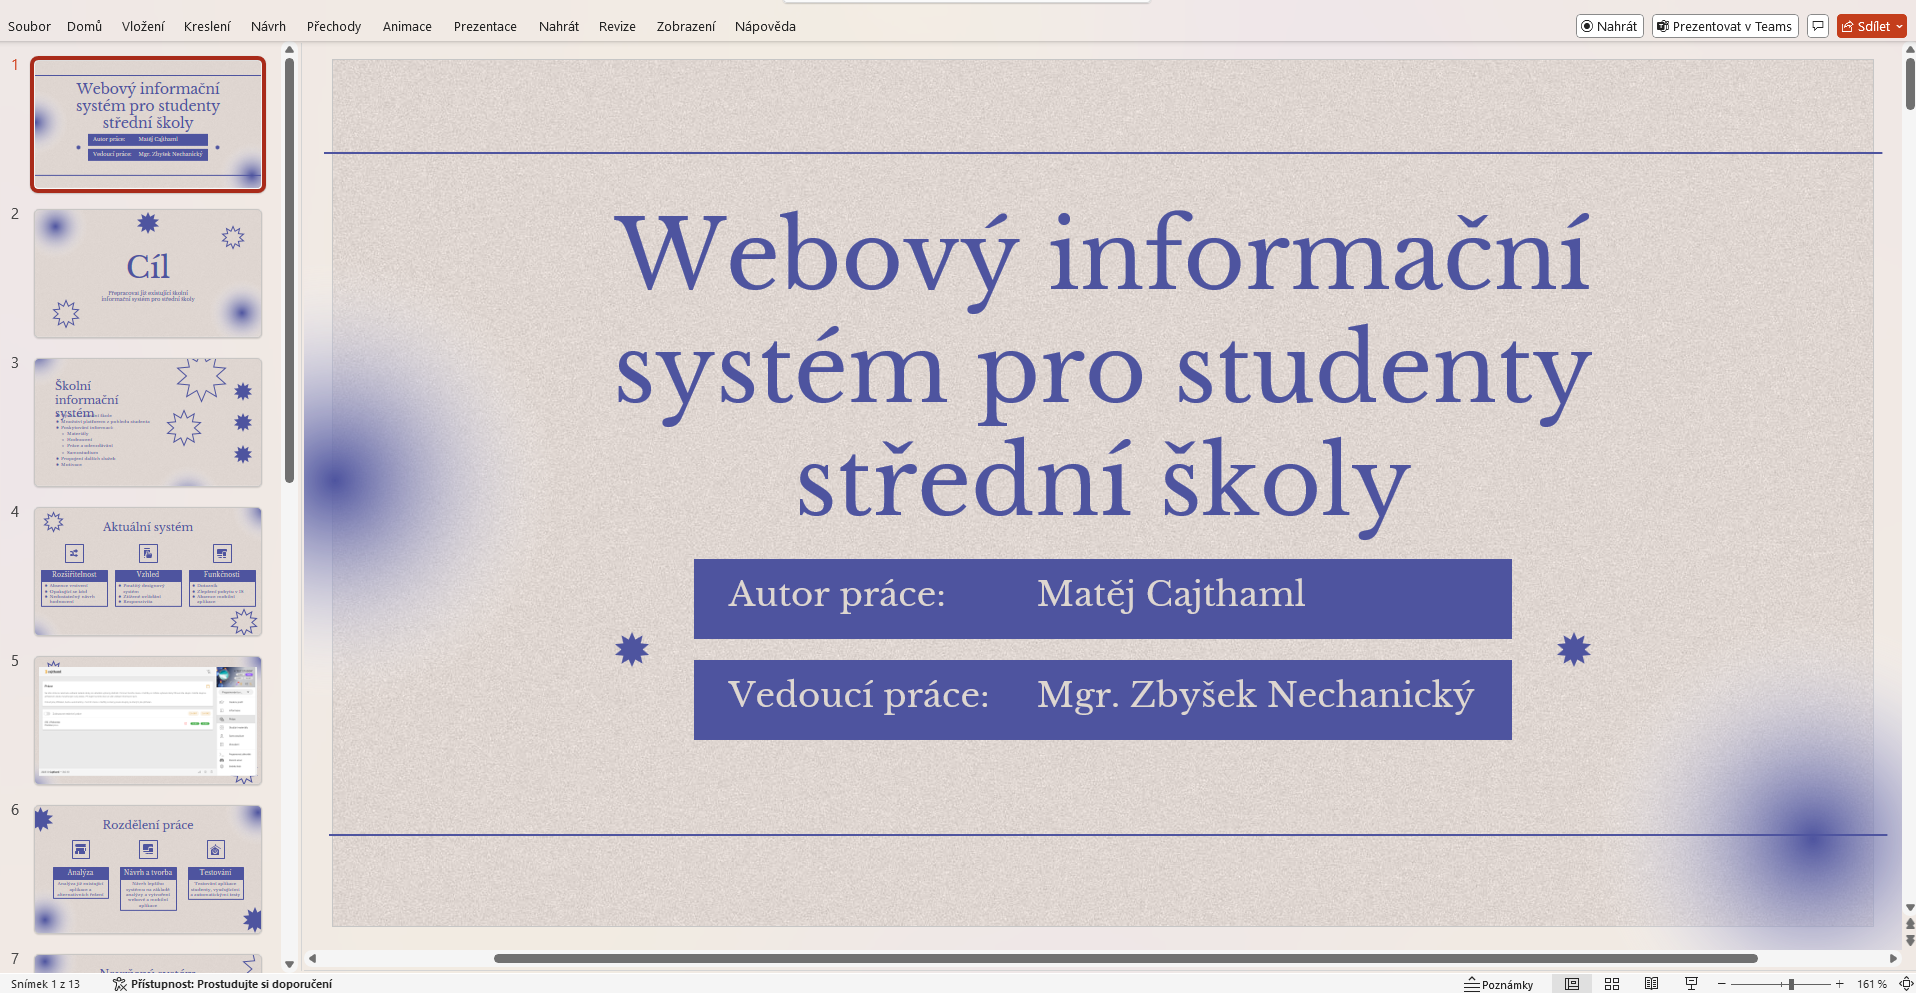
\includegraphics[width=0.8\textwidth]{media/03_analyza/powerpoint.png}
    \caption[Prezentace v~PowerPoint, pro státní závěrečnou zkoušku]{Prezentace v~PowerPoint, prezentace pro státní závěrečnou zkoušku (vlastní zpracování)}
    \label{fig:analyza/powerpoint}
\end{figure}


\subsection{Google Slides}\label{text:google_slides}

Google Slides~\cite{slides} je bezplatný webový nástroj pro tvorbu prezentací od společnosti Google. 
Hlavní přednosti spočívají v~možnostech snadné spolupráce více uživatelů v~reálném čase, neboť dokument lze sdílet a společně editovat odkudkoli.
Integrace s~ostatními službami Google (Disk, Dokumenty, Tabulky) umožňuje jednoduchý import a export různých typů souborů a díky tomu se výrazně usnadňuje týmová práce a přístup ke společným materiálům. 
Podobně jsou implementovány integrace s~komunitními rozšířeními ze služeb Google.
Ve výchozím stavu je služba zdarma, avšak pokročilé funkce a správa dat jsou často vázány na účet v~rámci Google Workspace~\cite{slides}, který mohou organizace platit v~rámci firemního nebo institucionálního předplatného. 

Výhodou je automatické ukládání na cloud, takže není nutné se obávat ztráty dat~\cite{slides}, a navíc je vše dostupné na více zařízeních, což usnadňuje vzdálený přístup k~prezentacím. 
Na druhou stranu je nezbytné mít stabilní připojení k~internetu a být obezřetný vůči ukládání citlivých údajů do cloudu, protože Google Slides shromažďuje metadata o~aktivitě uživatelů (například informace o~tom, kdo a kdy dokument editoval)~\cite{google_terms}, což může s~ohledem na soukromí a bezpečnost některým institucím či uživatelům vadit. 
Dále je možné, že prezentace vytvořené v~Google Slides nebudou stoprocentně kompatibilní s~PowerPointem a jinými nástroji zejména ve své interaktivitě a pluginy, což může způsobit problémy při přenosu mezi různými platformami. 
Nevýhodou jsou také omezenější pokročilé funkce, animace či grafické úpravy oproti PowerPointu nebo jiným specializovaným nástrojům. 

Google Slides nicméně celkově nabízí snadno použitelný a přístupný nástroj pro spolupráci a rychlou tvorbu prezentací, který uživatelům postačí pro většinu běžných scénářů, obzvláště tam, kde je důraz na flexibilitu, týmovou práci a okamžitý vzdálený přístup k~materiálům.


\subsection{RevealJS}\label{text:revealjs}

RevealJS~\cite{revealjs} je knihovna a framework, která dovoluje tvořit prezentace pomocí zdrojového kódu v~HTML. 
Výsledné prezentace jsou k~dispozici jako webová stránka, ve které se vykreslují jednotlivé snímky, mezi kterými lze plynule procházet. 
Velkou výhodou RevealJS je široká komunita, řada open-source pluginů a neomezené možnosti integrace multimediálního obsahu, od videí přes animace až po spustitelný kód. 
Nevýhodou může být různé zpracování, dokumentace a nastavení pluginů, které nemusí být vždy vzájemně kompatibilní, nutnost znalostí webových technologií a absence WYSIWYG editoru. 

Vytvořené prezentace je často nutné hostovat na cloudu, zejména pokud používají pluginy vyžadující serverové prostředí.
Společnost, která vytvořila RevealJS, taktéž vytvořila službu Slides.com~\cite{revealjs, slidescom}, umožňující tvořit prezentace pomocí editoru s~frameworkem RevealJS, s~prémiovými pluginy a automatickým cloudovým uložením, avšak tento nástroj je kódově uzavřený a placený. 

Osobně jsem RevealJS knihovnu již řadu let používal pro tvorbu prezentací pro své studenty, kteří ocenili možnost vytvářet v~prezentaci interaktivní prvky, jako je například kódový blok s~okamžitým zobrazením výsledku. 
Na obrázku~\ref{fig:analyza:revealjs-ukazka} je vidět příklad takové prezentace, kde je vlevo kód a vpravo výsledek zobrazený v~prohlížeči, což podporuje lepší pochopení učiva a aktivní zapojení studentů. 

Zajímavou funkcí jsou i~tzv. vertikální snímky, které umožňují nelineární strukturování prezentace, kdy se lze pohybovat nejen horizontálně, ale i~vertikálně v~rámci logických celků prezentace.
Celkově si uživatelé chválí i~možnost modularity těchto snímků a že je velmi jednoduché spojovat jednotlivé atomické skupiny do větších celků.


\begin{figure}[ht!]
    \centering
    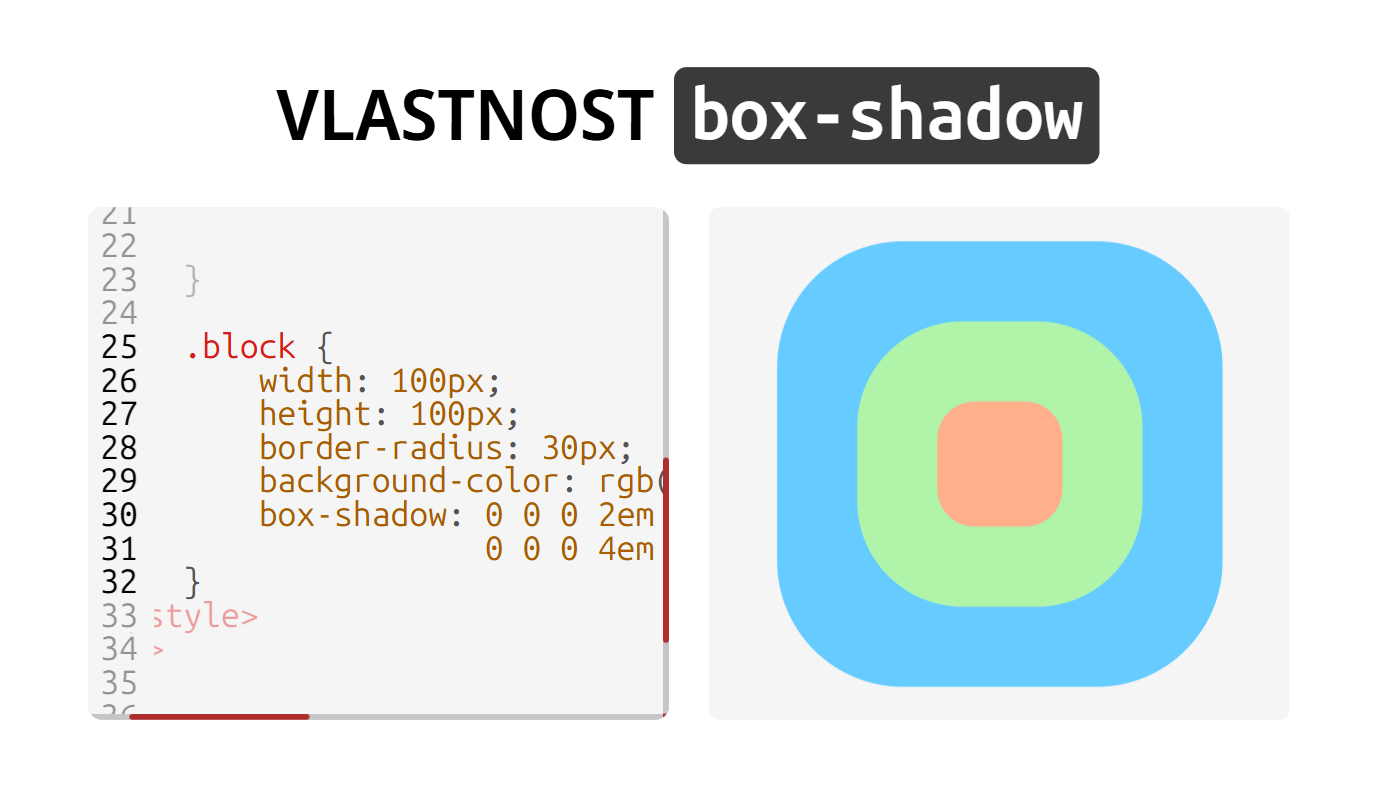
\includegraphics[width=0.9\linewidth]{media/03_analyza/revealjs.png}
    \caption[RevealJS prezentace s~rozdělením kódu a výsledku]{RevealJS prezentace s~rozdělením kódu a výsledku (vlastní zpracování)}\label{fig:analyza:revealjs-ukazka}
\end{figure}

\subsection{Beamer v~\LaTeX}

Beamer~\cite{beamer} je třída v~sázecím systému \LaTeX, která se zaměřuje na vytváření snímkových prezentací.
Nejvíce je Beamer společně s~\LaTeX~populární v~akademickém prostředí, zejména z~důvodu jednoduchého sazby matematických formulí a zápisu pomocí kódového jazyka, který leccos dovoluje. 

Zápis je ale zároveň to nejvíce nenáviděné na \LaTeX~\cite{latex_reddit}, a to zejména z~důvodu kryptických kódových chyb a různých zastaralých zápisů.
Vygenerované prezentace jsou taktéž statické a nedá se v~nich dělat jakákoliv interaktivita. 
Za částečnou interaktivitu jde počítat možnost generovat fragmenty snímků tak, že se na dalším zobrazí pouze následující část textu.
Ve výsledku se pro každý fragment do výsledného PDF vygeneruje další snímek.

Výhodou takovéto kódové generace je, že z~jednoho zdrojového kódu -- pro prezentaci -- se často dají tvořit taktéž skripta, a to tím, že přidáváme takové bloky kódu, které se vykreslí právě v~jednom nebo obou módech.
Další výhodou je řada knihoven, které již existují mnoho let, a které dovolují komplikované vizualizace a vykreslování.
Jedna z~nich je například knihovna TikZ. 

\section{Aplikace na grafickou tvorbu}\label{text:analyza/grafika}

Tato sekce se zaměřuje na nástroje, které umožňují snadno a rychle vytvářet vizuálně atraktivní materiály, ať už jde o~grafiky, ilustrace, uživatelská rozhraní či jiné kreativní prvky doplňující prezentace a vzdělávací materiály.

\subsection{Canva}\label{text:canva}

Canva~\cite{canva_website} je webová platforma pro rychlou a snadnou tvorbu grafických materiálů, jako jsou plakáty, letáky, sociální příspěvky či prezentace, s~bohatou nabídkou šablon, fontů a grafických prvků. 
Hlavní výhody Canva spočívají v~intuitivním uživatelském rozhraní~\cite{canva_recenze}, které je možná až příliš jednoduché, obrovské knihovně předpřipravených šablon a prvků, možnosti \enquote{drag-and-drop} úprav a snadné integraci multimédií.

Díky cloudovému prostředí umožňuje Canva týmovou spolupráci~\cite{canva_live_help, canva_live_features}, sdílení souborů v~reálném čase a přístup k~materiálům odkudkoli, přičemž většina základních funkcí je dostupná zdarma. 

Nevýhodou může být omezenější možnost zcela individuálního designu u~některých šablon, menší preciznost u~specifických grafických úprav a u~pokročilých funkcí je potřeba si zaplatit placenou verzi Canva~Pro. 
Přesto je aplikace Canva velmi oblíbená pro rychlou tvorbu vizuálně atraktivních materiálů i~mezi pedagogy, kteří nepotřebují pokročilé znalosti grafických programů a chtějí rychle připravit poutavé grafické materiály či prezentace.
Čeští pedagogové mají program Canva k~dispozici zdarma po ověření~\cite{canva_education}. Tento nástroj je mezi pedagogy velmi oceňován zejména právě pro jeho jednoduchost~\cite{canva_facebook}.

Canva má taktéž za svůj cíl vybudovat zodpovědnou firmu, a proto se zaměřují i~na školení svých uživatelů, jak tvořit kvalitní grafické materiály.
Tyto materiály, respektive kurzy, jsou zcela zdarma a tématy se zaměřují od logotypů, plakátů až ke tvoření kvalitních studijních materiálů pro specifické předměty.


\subsection{Figma}\label{text:figma_popis}

Figma~\cite{figma_website} je profesionální online nástroj pro design a prototypování uživatelských rozhraní, který se v~posledních letech stal standardem v~oblasti webového a aplikačního designu. 
Nabízí vektorový grafický editor, možnost vytvářet interaktivní prototypy a sdílet je v~reálném čase s~kolegy, což výrazně usnadňuje spolupráci v~týmech~\cite{figma_website}. 
Velkou předností Figma je její cloudové prostředí, ve kterém se změny ukládají automaticky a každý člen týmu vidí okamžité aktualizace, což zjednodušuje proces zpětné vazby a revizí. 

Nevýhodou může být vyšší křivka učení pro uživatele neznalé profesionálních grafických nástrojů a nutnost stabilního připojení k~internetu, aby bylo možné plně využít funkce Figma. 
Přesto Figma představuje výkonný a flexibilní nástroj, který může pedagogům a školám pomoci při tvorbě interaktivních rozhraní pro studijní materiály, e-learningové platformy či jiné digitální vzdělávací projekty.
Podobným problémem je omezený neplacený režim, který hodně omezuje počet a velikost projektů, a to včetně počtu současných editorů dokumentu.

Inspirativní částí Figma jsou velmi pokročilé možnosti editoru, jako je například interaktivní prototypování.
To zahrnuje například možnosti přepínání komponent či jednotlivých rámců.
Velké pozitivum je i~velké komunitní zapojení do prosperity aplikace pomocí tvorby komunitních rozšíření a šablon.

Figma se zaměřuje i~na tvoření poznámek či pláten~\cite{figma_figjam} ve své dceřiné aplikaci FigJam.
Tento nástroj je postaven na stejném editoru, jako používá hlavní aplikace.
Podobně Figma dovoluje pomocí různých šablon i~tvoření prezentací.
Tyto prezentace však postrádají řadu nepostradatelných funkcionalit, jako jsou například animační schopnosti a optimalizace na procházení snímky.

\section{Aplikace na tvorbu materiálů}\label{text:analyza/materialy}

Tato sekce představuje nástroje, jež umožňují připravovat a distribuovat výukové materiály v~podobě interaktivních prezentací, kvízů, vizuálních map či jiných vzdělávacích formátů.
Tyto nástroje tedy mají velmi podobné cíle jako aplikace, která má vzniknout z~téhle práce.
Hlavním cílem těchto aplikací je zefektivnit a zpestřit proces učení, zvýšit zapojení studentů a nabídnout pedagogům možnosti, jak obohatit svou výuku o~moderní a atraktivní formy obsahu.

\subsection{Genially}

Genially~\cite{genially} je online platforma pro tvorbu interaktivních materiálů, prezentací, infografik a dalších multimediálních podkladů, které mohou publikum aktivně zapojit do obsahu.
Platforma je navržena s~důrazem na jednoduchost použití, aby byla dostupná jak profesionálům, tak i~laikům.

Jednou z~klíčových vlastností Genially je možnost rychlého přidávání interaktivních prvků~\cite{genially}, jako jsou kvízy, hypertextové odkazy, animace a různorodý multimediální obsah. 
Tyto funkce nejen zvyšují zapojení studentů, ale také podněcují jejich motivaci k~učení skrze aktivní interakci s~obsahem. 
Tím se platforma stává nejen nástrojem pro prezentaci informací, ale také prostředkem pro výuku založenou na principu konstruktivistické pedagogiky~\cite{konstruktivismus}. 
% Konkrétní příklady interaktivních prvků zahrnují již zmíněné odkazy, kliknutí, řazení, kvízy, interaktivní aplikace uvnitř a mnoho dalšího.

Velkou předností Genially je jeho intuitivní rozhraní a široká škála připravených šablon.
Tyto šablony jsou navrženy s~ohledem na vizuální atraktivitu a dynamiku, což umožňuje rychlou tvorbu obsahu bez nutnosti pokročilých grafických znalostí.
Platforma tak poskytuje tvůrcům nástroje, které by jinak vyžadovaly~\cite{genially} komplexní software a odborné znalosti.

Genially je však placená služba, což může představovat značnou překážku pro vzdělávací instituce a jednotlivce s~omezenými finančními zdroji. 
Bezplatná verze nabízí pouze omezenou funkcionalitu a materiály vytvořené v~rámci této verze obsahují vodoznak.
Dále je export obsahu možný pouze u~placených tarifů, a to v~různých formátech, jako jsou PDF nebo HTML. 
Tato omezení mohou snižovat flexibilitu uživatele, který by chtěl svůj obsah sdílet, archivovat offline a nebo celkově více plánovat výuku. 
Zároveň nelze provádět vlastní úpravy kódu ani integrovat komunitní rozšíření, což je omezující pro uživatele, kteří by potřebovali pokročilé nebo zcela unikátní funkce.

Je třeba zmínit, že Genially jako firma je formálně napojena na platformu Canva~\cite{genially}, viz sekce~\ref{text:canva}, a tyto dvě služby sdílejí základ vizuálního editoru. 
Tento aspekt zvyšuje celkovou kvalitu uživatelského zážitku, protože editor se vyznačuje vysokou přehledností a snadnou manipulací s~obsahem. 
Z tohoto pohledu lze považovat Genially za nástroj, který efektivně staví na osvědčených principech uživatelského designu a zajišťuje širokou dostupnost profesionálních vizuálních standardů.

Na základě vlastních zkušeností jsem využil Genially pro tvorbu několika prezentací a vzdělávacích materiálů. 
Zatímco samotná tvorba byla rychlá a relativně bezproblémová, setkal jsem se s~určitými nedostatky, které ztěžovaly optimální využití platformy. 
Jedná se o:

\begin{itemize}
    \item Omezenost obsahu, kdy počet různých prvků, které lze vložit do plátna, je opravdu malý a obecně se tím pádem vytvořené materiály hodí pouze na hodně obecné předměty. Pro informační technologie neobsahuje aplikace skoro nic vhodného.  
    \item Limitace \enquote{klávesnice}, kdy spousta věcí lze dělat pouze v~uživatelském prostředí pomocí klikání. 
    \item Omezené možnosti exportu, jelikož hotové prezentace nelze jednoduše stáhnout ve formátu PDF nebo PPTX bez placené verze. To omezuje offline využití materiálů.  
    \item Pomalá odezva editoru u~složitějších projektů, kdy větší množství objektů způsobuje zpomalení při úpravách a načítání.  
\end{itemize}

Problémy jsem měl i~při prezentování vytvořených materiálů. 
Studenti měli taktéž problémy vytvořené \enquote{aplikace} používat. 
Sdílené materiály nemají moc intuitivní rozhraní a interaktivní prvky, které lze vložit, nemají moc dobrý uživatelský zážitek.

Na Genially jsem mezi českými učiteli nenašel moc objektivních hodnocení.
Od platformy Učíme online existují webináře a kurzy~\cite{genially_ucimeonline}, které celou aplikaci představují.
Podobně lze najít v~různých komunitách na sociálních sítích i~v~nesouvisejících skupinách~\cite{canva_facebook} různé názory, které zejména zmiňují složitou tvorbu lekcí.

\subsection{Mentimeter}

Mentimeter~\cite{mentimeter} je webová aplikace určená pro interaktivní zapojení publika prostřednictvím online hlasování, dotazníků, kvízů, slovních mraků, průzkumů a anket. 
Umožňuje učitelům a přednášejícím získávat okamžitou zpětnou vazbu od studentů, což napomáhá identifikovat oblasti nepochopení, zvýšit míru interakce a podporovat aktivní účast na výuce. 

Velkou předností Mentimeter je jeho uživatelská přívětivost, široká nabídka interaktivních formátů, kompatibilita s~mobilními zařízeními a snadná integrace do výukových scénářů, přičemž výsledky lze ihned zobrazit na obrazovce. 
Vzhledem k~tomu, že Mentimeter se zaměřuje zejména na interakci a aktivní zapojení publika, nikoliv na obsah samotný, nenabízí~\cite{mentimeter_review} mnoho grafických funkcí pro tvorbu složitých nebo vizuálně bohatých materiálů. 
Podobně vyučující uvádí problém s~rozdělením odpovědí na jednotlivé studenty či s~velmi omezenou neplacenou verzí.

Stejně jako Genially zde chybí komunitně tvořené rozšíření a detailní možnosti kódových úprav, avšak pokud je cílem zvýšit interaktivitu a okamžitou odezvu od studentů, Mentimeter tento úkol splní velmi dobře.

Mentimeter jsem aplikoval několikrát ve výuce a splnil to, co jsem očekával, a to, že se zvýšila interaktivita ve výukové skupině. 
Velkým problémem je opravdu to, že obsah nejde upravovat natolik, aby šlo vytvořit originální a graficky rozlišitelný obsah. 
V aplikaci taktéž velmi chybí grafické možnosti, na jednotlivé snímky lze vložit pouze jeden interaktivní prvek s~jednotkami grafických variací.

\subsection{Prezi}

Prezi~\cite{prezi} je prezentační nástroj, který se odlišuje od klasických lineárních prezentací svou nelineární strukturou.
Místo jednotlivých snímků pracuje Prezi s~jedním velkým plátnem, na němž lze rozmístit text, obrázky, videa a další obsah do logických celků, mezi kterými lze dynamicky přecházet pomocí pohyblivých či přibližovacích efektů.
Aplikace je tedy takovým velkým plátnem, v~podstatě jednou myšlenkovou mapou.
To však omezuje její použití na pouze jeden konkrétní případ způsobu výuky -- obyčejné prezentace, plakáty a další materiály zde vypadají velmi zvláštně.

Hlavní předností Prezi je vizuální atraktivita, flexibilita v~organizaci obsahu a neobvyklý způsob zobrazení témat, který může pomoci udržet pozornost posluchačů a lépe vyjádřit souvislosti mezi jednotlivými informacemi. 

Nicméně Prezi nenabízí výrazně interaktivní prvky pro zapojení studentů, nepodporuje komunitně tvořená rozšíření a soustředí se především na propojení vytvořených témat společně s~vizuálním aspektem prezentací, nikoliv na interakci či možnost programových úprav.

Prezi jsem se snažil použít, jejich editor je však velmi zvláštní a odbočuje od známých standardů UI a UX.
Prezi je taktéž placená aplikace a omezuje použití jakýchkoliv pokročilých obsahů, a tedy použití je bez toho prakticky nemožné a slouží spíše jako ukázka možností.

\section{Sumarizace knihoven a nástrojů}

V tabulce~\ref{tab:porovnani_prezentaci} je sumarizovaná sekce~\ref{text:analyza/prezentace}, která se zaobírá různým softwarem na tvorbu prezentací.
Z tabulky vyplývá, že zatímco PowerPoint a Google Slides nabízejí jednoduché a intuitivní použití, RevealJS a Beamer vyžadují znalosti kódování, ale umožňují větší flexibilitu.
Největší rozdíly jsou v~interaktivitě, přístupnosti a v~dostupnosti pokročilých funkcí, přičemž žádný z~těchto nástrojů není jednoznačně nejlepší pro všechny uživatele.


\begin{table*}[ht!]
    \centering
    \resizebox{\textwidth}{!}{%
    \begin{tabular}{|p{2.3cm}||p{2.7cm}|p{2.8cm}|p{3cm}|p{3cm}|}
        \hline
        \textbf{Funkce} & \textbf{PowerPoint} & \textbf{Google Slides} & \textbf{RevealJS} & \textbf{Beamer} \\
        \hline        \hline
        Cena                & Placený & Zdarma & Zdarma & Zdarma \\\hline
        Prémiové funkcionality & Ano & Ano & Ano (Slides.com) & - \\\hline
        Přístupnost         & Desktop/Web & Web & Web & Lokální \\\hline
        Spolupráce          & Ano & Ano & Git/Cloud/IDE & Git/Cloud/IDE \\\hline
        Interaktivita       & Základní & Základní & Vysoká & Žádná \\\hline
        Šablony             & Bohaté & Bohaté & Flexibilní & Základní \\\hline
        % Podpora formátů     & PPTX &  & Webová &  \\\hline
        Používání           & Intuitivní & Intuitivní & Kódování HTML, CSS a JS & Obtížné \\\hline
        Unikátní vlastnosti & Integrace s~Office & Cloudové ukládání & Interaktivní prvky & Možnost skript\\\hline 
    \end{tabular}%
    }
    \caption{Porovnání aplikací pro tvorbu prezentací}
    \label{tab:porovnani_prezentaci}
\end{table*}


V tabulce~\ref{tab:porovnani_grafika} je sumarizovaná sekce~\ref{text:analyza/grafika}, která se zaobírá různým softwarem na tvorbu grafických materiálů, prezentací a návrhů aplikací.
Canva se vyznačuje jednoduchostí a rychlou tvorbou obsahu, zatímco Figma nabízí pokročilé nástroje a interaktivní prototypování, ale je náročnější na osvojení. Oba nástroje mají komunitní šablony, avšak Canva se zaměřuje spíše na rychlou grafickou úpravu, zatímco Figma cílí na UI/UX design s~větší možností spolupráce v~reálném čase.


\begin{table*}[ht!]
    \centering
    \resizebox{\textwidth}{!}{%
    \begin{tabular}{|p{2cm}||p{6cm}|p{6cm}|}
        \hline
        \textbf{Funkce} & \textbf{Canva} & \textbf{Figma} \\
        \hline \hline
        Cena & Zdarma vs. Canva Pro & Zdarma vs. Figma Pro \\\hline
        Zaměření & Grafické materiály, prezentace & UI/UX design, prototypování \\\hline
        Přístupnost & Webová aplikace, mobilní verze & Webová aplikace, desktopová aplikace \\\hline
        Spolupráce & \multicolumn{2}{|c|}{Ano, v~reálném čase} \\\hline
        Interaktivita & Omezená (základní animace) & Pokročilá (interaktivní prototypy) \\\hline
        Šablony & Bohatá knihovna & Šablony a komunitní rozšíření \\\hline
        Používání & Intuitivní, drag-and-drop & Náročnější, vektorový editor \\\hline
        Unikátní vlastnosti & Snadné použití, rychlá tvorba grafiky & Pokročilé nástroje, FigJam pro poznámky \\\hline
        Omezení & Méně přizpůsobitelné šablony, nutnost placené verze pro některé funkce & Vyšší křivka učení, omezený neplacený režim \\\hline
    \end{tabular}%
    }
    \caption{Porovnání aplikací na grafickou tvorbu}
    \label{tab:porovnani_grafika}
\end{table*}

V tabulce~\ref{tab:porovnani_materialy} je sumarizovaná sekce~\ref{text:analyza/materialy}, která se zaobírá aplikacemi, které slouží k~tvorbě materiálů.
Genially umožňuje tvorbu interaktivních vzdělávacích materiálů, ale omezuje uživatele placenými funkcemi a šablonovým systémem.
Mentimeter je skvělý pro zapojení studentů do výuky prostřednictvím kvízů a hlasování, ale postrádá pokročilé grafické možnosti. 
Prezi nabízí inovativní způsob prezentování obsahu, ale kvůli své specifické struktuře není univerzálním řešením pro všechny výukové situace.


\begin{table*}[ht!]
    \centering
    \resizebox{\textwidth}{!}{%
    \begin{tabular}{|p{2.3cm}||p{3.5cm}|p{3.5cm}|p{3.5cm}|p{3cm}|}
        \hline
        \textbf{Funkce} & \textbf{Genially} & \textbf{Mentimeter} & \textbf{Prezi} \\
        \hline \hline
        Cena & \multicolumn{3}{|c|}{Zdarma, placená verze s~prémiovými funkcionality} \\\hline
        Zaměření & Interaktivní prezentace, infografiky & Interaktivní hlasování, kvízy & Prezentační software s~nelineární strukturou \\\hline
        Přístupnost & Webová aplikace & Webová aplikace & Webová aplikace, desktopová verze \\\hline
        Interaktivita & Klikací prvky, kvízy, multimédia & Hlasování, dotazníky, slovní mraky & Zoom efekty, pohyblivé přechody \\\hline
        Šablony & Bohatá knihovna & Omezené varianty & Specifické pro Prezi formát \\\hline
        % Používání & Intuitivní & Snadné použití, rychlá odezva & Nestandardní ovládání, vyžaduje zvyk \\\hline
        Export materiálů & Pouze v~placené verzi (PDF, HTML) & Omezené exportní možnosti & Placená verze nutná pro export offline \\\hline
        Unikátní vlastnosti & Kombinace vizuálních prvků a interaktivity & Okamžitá zpětná vazba od studentů & Nelineární prezentace, zoom efekt \\\hline
        Omezení & Omezená přizpůsobitelnost, placené funkce & Grafická jednoduchost, pouze jeden interaktivní prvek na snímek & Malé možnosti interakce, zvláštní UX \\\hline
    \end{tabular}%
    }
    \caption{Porovnání aplikací pro tvorbu materiálů}
    \label{tab:porovnani_materialy}
\end{table*}

Z analýzy jednotlivých kategorií aplikací vyplývá, že neexistuje jeden nástroj, který by splňoval všechny potřeby uživatelů, což značně komplikuje výběr ideálního řešení. Každá aplikace se zaměřuje na specifickou oblast a přináší své výhody i~omezení, což znamená, že uživatelé často musí kombinovat více nástrojů. 
Klíčovým problémem u~většiny analyzovaných aplikací je závislost na placených verzích, omezená přizpůsobitelnost nebo nedostatek interaktivity.
Pro ideální nástroj by bylo zásadní nabídnout dostatečnou míru flexibility, široké komunitní rozšíření a otevřenost vůči uživatelským úpravám, což by umožnilo efektivnější a univerzálnější využití v~různých vzdělávacích scénářích.

\section{Způsoby vykreslování na webových stránkách}\label{text:vykreslovani}

Většina grafických aplikací potřebuje nějakým způsobem vykreslovat obsah programu.
Na webových stránkách jsme vykreslováním velmi omezeni.
Existují však různé alternativy zápisu a tvorby za pomocí různých prvků v~HTML standardu.
Tyto způsoby v~této sekci rozeberu i~s~jejich plusy a mínusy.

\subsection{HTML prvky}\label{text:vykreslovani/html}

HTML je základní značkovací jazyk~\cite{uzayr2022frontend} pro tvorbu webových stránek. 
V rámci vykreslování obsahu na webu jsou k~dispozici různé HTML prvky, které umožňují zobrazení statických i~dynamických dat.
S pomocí CSS je možné tyto prvky skoro nelimitovaně~\cite{uzayr2022frontend} stylovat a pozicovat.

Použití tohoto způsobu je velmi jednoduché, protože je to v~podstatě tvoření webové stránky.
% Problém bývá s~interaktivitou~\cite{uzayr2022frontend}, že i~mimo tohle potř s~prvky pracovat a díky Document Object Model (DOM) je toto možné provést.
Kvůli častým změnám a závislostem proměnných na šablonách, resp. konkrétních prvcích je často nutné vytvořit tzv. virtuální DOM.
Virtuální DOM tvoří a emuluje to, co dělá DOM, jen s~tím rozdílem, že program má nad celým vykreslováním, závislostmi celou kontrolu.
Virtuální DOM je klíčovou věcí pro skoro všechny moderní frameworky~\cite{uzayr2022frontend} na webových stránkách, jako React, Vue a tisíce dalších.

HTML, CSS, JS a (virtuální) DOM je poté možným způsobem, jak vykreslovat skoro jakýkoliv obsah na webové stránce a zároveň nad tím mít kompletní kontrolu.
Problémem bývá omezenost box-modelu a způsob pozicování, což může v~některých případech limitovat flexibilitu při vytváření složitějších layoutů nebo interaktivních prvků. 
Box-model vychází z~pevně dané šířky, výšky, okrajů, odsazení a okrajů okna pro prohlížeč, což může být komplikováno v~případě, kdy je potřeba pracovat s~dynamickým a variabilním obsahem. 
I když CSS nabízí pokročilé metody, jako flexbox nebo grid, které značně zlepšují~\cite{uzayr2022frontend} flexibilitu layoutu, stále existují případy, kdy HTML prvky samy o~sobě nestačí k~dosažení požadovaného chování bez použití komplexního skriptování a dalších technologií.
Vykreslování je často pomalé s~velkým počtem prvků díky (ne)optimalizacím prohlížečů.

Tento způsob používá velmi mnoho služeb a knihoven, jako ukázku uvádím například zmíněnou knihovnu RevealJS (viz sekce~\ref{text:revealjs}).

\subsection{Canvas}

Canvas je prvek z~HTML~\cite{canvashtml5, uzayr2022frontend}, který je sémanticky a definičně určen k~vykreslování komplexního grafického designu, her a podobných věcí.
Do Canvas se vykresluje pomocí JS (případně jiné jazyky, viz sekce~\ref{text:webassembly}) a to dovoluje měnit jednotlivé pixely, překreslovat je a tvořit animace.
Klasické módy Canvas jsou však omezené a často se aplikace rozhodnou používat nástavbovou knihovnu WebGL~\cite{canvashtml5}, která místo nekomplexního systému kreslení pixelů dovoluje komunikovat s~GPU.
Dovoluje totiž definovat shadery~\cite{canvashtml5} pro GPU a spoustu dalších nastavení pro renderování obrazu.
Můžeme tedy tvořit velmi komplexní věci, optimalizovat je a webovou stránku ovládat jako jakýkoliv jiný obsah. 

Nevýhodou však může být složitost implementace~\cite{canvashtml5} a potřeba znalosti programování pro shadery.
V podstatě není nic dalšího definováno a i~obyčejný okraj je nutné složitě naprogramovat.
Existují samozřejmě knihovny (např. ThreeJS) které pro nás definují~\cite{canvashtml5} shadery předem a dovolují další věci, jako např. načítání obrázků či modelů.
Navíc takto komplexní výpočty potřebují silnější zařízení, na kterých webová stránka běží.

I když je Canvas sémanticky popsán~\cite{canvashtml5}, veškerý vykreslený obsah nikoliv a je tedy velmi těžké sémanticky určit, co se vlastně vykresluje.

Kvůli náročnosti tento způsob používá méně služeb. 
Ze zmíněných uvádím jako ukázku například program Figma (viz sekce~\ref{text:figma_popis}).
Jejich způsob vykreslování je velmi kvalitní a je vidět, že do aplikace investovali velmi mnoho zdrojů.
Jejím cílem je ale být grafický nástroj a přesnost všeho je pro jejich uživatele důležitá.

\subsection{SVG}

Scalable Vector Graphics (SVG) slouží k~definování vektorových prvků~\cite{svg_css_html}, které se mohou jednoduše vykreslovat na webové stránce.
To dovoluje jednoduše používat daný vytvořený \enquote{obrázek} v~jakémkoliv rozlišení.
Moderní SVG dovolují dovnitř jako prvek vkládat i~rastrové obrázky a další cizí objekty~\cite{svg_css_html, uzayr2022frontend}, které se poté poměrně jednoduše vykreslují.

Veškeré prvky by se tedy pro vykreslování obsahu mohly definovat v~jednom velkém SVG, kde by každá stránka či snímek byl jedno SVG, které by v~sobě mělo jednotlivé prvky.

Mezi nevýhody tohoto systému patří zejména problém s~vykreslováním, protože rasterizace vektorového obrazu je drahá operace~\cite{svg_css_html}, a to zejména ve webovém prostředí.
Další omezení je i~v~tom, co s~danými prvky poté jde dělat, protože tento způsob limituje to, co můžeme na dané prvky nastavit jako odchytávače události a respektive vůbec jaké události můžeme vkládat.
Hodně to ubírá na možné interaktivitě.
Dále se uvádí~\cite{svg_css_html} jako nevýhoda kompatibilita mezi prohlížeči.

Mezi výhody patří velké možnosti filtrů a definic, jednoduchý možný export a jednoduché transformace.
Tyto věci však umí i~jiné varianty a nic navíc tento způsob nepřináší.

Toto vykreslování používají ze zmíněných služeb například Google služby, resp. Google Slides (viz sekce~\ref{text:figma_popis}).

\section{Komunitní rozšíření}\label{text:community_plugins}

Cílem práce je vytvořit platformu, která bude podporovat komunitní rozšíření.
K tomu bude velmi důležité navrhnout, jak se toto rozšiřování bude realizovat.

V této sekci je sepsáno, jak komunitní rozšíření řeší jiné existující služby a knihovny.

\subsection{Google služby}

V sekci~\ref{text:google_slides} jsem uvedl, že Google Slides integrují komunitní rozšíření -- úpravy platformy pomocí tzv. pluginů.
Tyto pluginy se používají tím, že uživatel v~aplikaci nalezne tlačítko se správou rozšíření, ve kterém vybere rozšíření, které chce aktivovat.
Aktivací se spustí řada skriptů, se kterými poté samotná aplikace Google Slides komunikuje a zajišťuje danou funkcionalitu.

Tyto skripty mohou definovat~\cite{google_apps} například:

\begin{description}
    \item[API] Komunikovat s~API Google Slides, tedy např. přidávat a modifikovat obsah jednotlivých snímků, přidávat snímky a nebo poskytnout přídavná okna s~dalším obsahem.
    \item[Události] Zachytávat se na události a reagovat na ně skrz výše uvedené API.
    \item[Menu] Vytvořit speciální položky v~navigaci, které budou dělat konkrétní změny.
\end{description}

Na spouštění skriptů uvnitř aplikace Google používá vlastní nástavbu jazyka JavaScript~\cite{google_apps}.
Tento jazyk a skripty v~něm vytvořené se zásadně spouští na jejich serverech v~emulátoru JavaScriptu tak, aby mohli jasně omezovat~\cite{google_apps} k~čemu má daný skript práva. 
Mezi omezení patří např. omezení volání požadavku, přístup k~tokenům a dalšímu.
Proto se nevolají skripty na klientské části, tedy není možné vytvořit emulátor, který poběží v~bezpečném prostředí.
Alternativou v~moderních prohlížečích je WebAssembly, které by něco takového mohlo dovolovat.
Tímto se budu zaobírat v~sekci~\ref{text:webassembly}.

Na internetu jsem hledal názory na tento způsob tvorby pluginů~\cite{google_apps_script_redit} a jeden z~největších problémů, na které uživatelé píší hodnocení, je právě omezenost spouštěče kódu.
Vzhledem k~tomu, že se pouští na serveru, je velmi limitována možnost měnit samotné HTML v~prohlížeči a tedy i~v~prezentacích.
Pluginy jsou tedy velmi často omezené pouze na volání API a přidávání základních prvků, které ale nedovolují velké možnosti modifikace.
Možnosti jsou ale přesto velké, nevýhoda je, že je nutné mít vlastní server, umět jasně pracovat se zabezpečením Google a hlavně se chytře vyhnout, resp. přizpůsobit se těmto omezením.

Podobně taktéž fungují další služby od společnosti Google.
Většina aplikací poté specializuje své API, aby sloužilo konkrétní službě.
Jejich platforma na skripty -- Apps Script je stále stejná~\cite{google_apps_script_redit, google_apps} pro všechny služby.

\subsection{RevealJS}

Bezpečnost rozšíření v~RevealJS se nemusí až tak řešit, protože je jejím správcem již programátor.
Rozšíření se tvoří tak, že je vytvořen JS soubor, který se importuje při inicializaci prezentace pomocí RevealJS.
Tento kód si poté knihovna zaháčkuje, jak je potřeba, a plugin odpovídá na vše, co je potřeba.
Často knihovny dělají věci okolo tím, že vkládají obsah na stránku mimo vědomí knihovny, upravují jednotlivé funkce uvnitř a podobně.

Mezi ukázky pluginů patří například napojení knihovny \texttt{mermaidjs} pro vykreslování grafů, přiblížení při kliknutí nebo například načítání externího kódu ze souboru pro zobrazení v~prezentaci.

Tato rozšíření často nemají žádný důvod zneužít důvěry instalace a pokusit se napadnout prezentaci.
Často totiž není ani co za data vzít, protože jsou stránky hostované v~nějakém hostingu, ve kterém se uživatel nepřihlašuje a nemá v~něm žádná data.
To, co uživatel do prezentace nainstaluje, je zcela na něm.

K RevealJS patří služba Slides.com~\cite{slidescom} (viz sekce~\ref{text:revealjs}).
Tyto stránky již dovolují stránky sdílet, mají editor a vzhledem k~tomu, že se již na stránce přihlašuje, sbírají se informace, je nutné, aby stránky omezily možná bezpečnostní rizika.
Proto platforma implementuje veškeré věci pomocí vlastních zabezpečených pluginů~\cite{slidescom} a jakékoliv věci ze třetích stran není možné používat.
Platforma ale implementuje řadu věcí a prezentace jsou použitelné.

\subsection{Figma}\label{text:figma}

Figma je velmi populární nástroj (viz sekce~\ref{text:figma}), který taktéž implementoval komunitní rozšíření~\cite{figma_website}.
Přístup vývojářů ke komunitnímu rozšíření je velmi veřejný a díky jejich blogu~\cite{figma_plugins_blog} je vidět řadu důvodů ke zvážení každé možnosti.
Figma svými tzv. pluginy zajišťuje rozšiřitelnost platformy, resp. zjednodušení používání aplikace.
Mezi ukázky takových pluginů patří například různé možnosti vkládání ikon, šablon, ale i~komplexní systémy na práci uvnitř editoru, jako hlasování v~návrzích.

Pluginy se zejména zaměřují na práci v~editoru, a proto některá rozhodnutí nejsou pro práci relevantní.
Při implementaci~\cite{figma_plugins_blog} se zaměřili na různé aspekty práce a způsoby spouštění nedůvěryhodného kódu, o~kterých budu mluvit později.

Mezi její zvažované přístupy patřilo Iframe, Realms, WebAssembly a další.
Každý přístup měl pro a proti, proto se nakonec rozhodli z~dvou užších možností -- Realms a WebAssembly -- přistoupit na Realms.
Jejich návrh platformy avšak dovoloval skoro bezpracné změnění způsobu volání kódu díky abstrakci.
To taktéž velmi rychle využili díky zranitelnosti Realms a i~když volání WebAssembly nebylo lepší v~celkovém porovnání, rozhodli se na něj přejít.
Jediná velká nevýhoda Realms je právě to, že daný kód běží ve stejném okně jako zbytek stránky a třeba i~jeho zpomalení (nezáměrné i~záměrné) může způsobit zaseknutí celé stránky.
Pro lepší bezpečnost je obecně počítat s~tím, že se ze systému, kde je kód uzavřen, může kód dostat.

Mimo jiné platforma pro každou možnost zvažovala~\cite{figma_plugins_blog, figma_website} řadu kritérií a specifikací. 
Níže je takový seznam, který může pomoci rozhodnout mezi správným přístupem:

\begin{itemize}
    \item Bezpečnost takové implementace, rizika opuštění kontrolovaného prostředí.
    \item Jednoduchost psaní skriptů a i~samotná implementace skriptů.
    \item Prostředky na spuštění takového kódu tak, aby to nebylo příliš náročné na zařízení.
    \item Kde spuštění probíhá, jak moc je možné systému věřit.
    \item Zpomalení spuštění skriptů a jeho reakce na události.
    \item Možnosti kódování a jeho jazyk.
\end{itemize}

\section{Spouštění nedůvěryhodného kódu}\label{text:anaylza/spousteniNeduveryhodnehoKodu}

Ze sekce~\ref{text:community_plugins} je očividné, že pro funkční a komplexní možnosti rozšíření jakékoliv aplikace je nutné vytvořit skriptovací platformu, která bude dovolovat spouštění nedůvěryhodného kódu.
Nedůvěryhodný kód jsou komunitní pluginy, které budou dovolovat programátorům upravovat stav aplikace a reagovat na možné události.

Ze stejné sekce vyšlo najevo, že čím více se toto spouštění omezuje, tím menší je využitelnost rozšíření vytvořených pro danou platformu.
Cílem této sekce je analyzovat možné způsoby spouštění nedůvěryhodného kódu a jejich výhody a nevýhody.

\subsection{Základní přístupy}

Uvnitř webových stránek díky podpoře JavaScriptu ve všech prohlížečích se lze bavit o~základních přístupech k~spouštění neověřeného kódu.
Jedná se o~evaluaci (\texttt{eval}) a o~domény (\texttt{Realms}).

Přímá evaluace je funkce~\cite{eval} z~JS, která dovoluje spustit jakýkoliv napsaný JS kód a získat z~něj výsledek.
To dovoluje spuštění v~podstatě jakéhokoliv skriptu v~prohlížeči.
Problém v~tomto přístupu je v~tom, že nelze jakkoliv omezit, k~čemu má spuštěný kód přístup~\cite{eval, shadowrealms, figma_plugins_blog}.
Tedy má přístup ke všemu.
Omezení se dá pokusit vytvořit pomocí např. struktury \texttt{with}, která umí změnit kontext \texttt{this}.
To lze však velmi jednoduše obejít např. pomocí přístupu k~prototype.
Tento způsob je tedy pro nedůvěryhodný kód nevhodný.

Alternativou k~\texttt{eval} je využití \texttt{Realms}, což je mechanismus poskytovaný specifikací ECMAScript (prostřednictvím návrhu TC39)~\cite{shadowrealms_propsal}. 
\texttt{Realms} umožňují vytvořit izolovaný běhový kontext, kde spuštěný kód nemá přímý přístup k~objektům a funkcím globálního kontextu hlavní aplikace~\cite{shadowrealms_propsal, shadowrealms}.
Každý \texttt{Realm} obsahuje svou vlastní kopii globálního objektu a základních vestavěných knihoven, což ztěžuje únik kódu mimo sandbox.
Přestože se jedná o~bezpečnější variantu oproti \texttt{eval}, má \texttt{Realms} své omezení, například v~podobě složitosti při komunikaci mezi hlavním a izolovaným kontextem. 
Další problém s~\texttt{Realms} je ten, že kód běží na jednom vlákně společně se zbytkem stránky a tak zásek v~tomto kódu způsobí zaseknutí celé webové stránky.

Způsob pomocí \texttt{Realms} původně zvažovali a implementovali vývojáři platformy Figma~\cite{figma_plugins_blog}.
V sekci~\ref{text:figma} je popsán postupný vývoj této platformy a to, jak se rozhodla z~\texttt{Realms}, kvůli svým kritickým chybám, přejít na WebAssembly.

\subsection{Iframe}

Iframe je sémantický tag v~HTML, který je určen pro vkládání stránky do stránky.
Iframe je velmi zabezpečený, protože pokud nejsou stránky ze stejné domény~\cite{iframe, figma_plugins_blog}, tak spolu nemohou komunikovat.
Vnější a ani vnitřní stránka tedy nemůže přečíst obsah a jakákoliv jiná data z~druhé stránky.
Jediná možná komunikace je pomocí tzv. messagingu, kde si mezi sebou mohou stránky vyměňovat jednoduché textové zprávy.

Iframe má taktéž kvůli zabezpečení tzv. nulový (\texttt{null}) origin pro CORS~\cite{iframe, figma_plugins_blog}.
To omezuje, resp. neguje, nastavení webových stránek pro ochranu uživatelů.
Zabezpečení je celkově ale velmi stabilní a to díky častým updatům prohlížečů.
Z iframe se v~podstatě nedá utéct, ale samozřejmě existovaly funkční pokusy o~prolomení, např. se jedná o~chybu s~protokolem prohlížeče~\cite{iframe_vuln}.
Obecně se považuje za velmi stabilní ochranu, které můžeme věřit díky skvělé práci skoro všech prohlížečů.

Iframe se nejčastěji používá na omezení nedůvěryhodného HTML kódu~\cite{iframe}.
Bez omezení by vložený kód z~rozšíření mohl utéci z~daného přiřazeného prvku a taktéž volat jakýkoliv kód jako stránka.
To by mohlo vést k~získání cookies či jiných lokálních souborů a tedy ke kompromitaci dat.

Tento způsob se nehodí používat na obecné skriptování -- je totiž velmi závislé pouze na předávání dat mezi oknem a danou stránkou, což je velmi limitující.

\subsection{Spuštění v~emulátoru}

Jednou z~možností, jak bezpečně spouštět nedůvěryhodný kód, je jeho izolace v~samostatném procesu. 
Tento přístup zajišťuje, že kód nemá přímý přístup ke zdrojům hlavní aplikace. 
Pro zvýšení bezpečnosti je nutné využít nástroj \texttt{chroot}, který omezuje přístup spuštěného procesu pouze na konkrétní adresářovou strukturu.

Existují specializované knihovny, jako například \texttt{vm2} nebo \texttt{isolated-vm} pro JS, které umožňují vytvoření izolovaných prostředí pro spouštění kódu. 
Tyto knihovny však nejsou univerzálně použitelné, zejména v~prostředí webových prohlížečů, kde nejsou podporovány. 
Tím pádem nelze tento přístup nasadit v~případech, kdy má být kód spuštěn přímo v~uživatelském prohlížeči.

Navíc v~minulosti existovaly takové zranitelnosti, které mohly umožnit obejití těchto omezení, což může vést ke kompromitaci aplikace.
A to je na serveru velmi nežádoucí.
Je proto nezbytné pravidelně aktualizovat používané knihovny a sledovat nové bezpečnostní postupy.

Hlavním problémem tohoto přístupu je komunikace mezi izolovaným procesem a hlavní aplikací. 
Vzhledem k~oddělení prostředí je komunikace omezená na asynchronní předávání zpráv, což přináší zásadní omezení. 
Například skript nebo plugin spuštěný v~tomto režimu nemůže v~reálném čase ovlivňovat stránku, což znemožňuje implementaci dynamických interakcí, jako je přidání prvku na stránku po kliknutí. 
Implementace něčeho takového by měla velmi velké zpoždění, a to se pro prezentační program nehodí.

Alternativou k~samostatným procesům je spuštění nedůvěryhodného kódu v~kontejnerech, například pomocí Dockeru. 
Tento přístup poskytuje vyšší úroveň izolace~\cite{docker}, protože kontejnery mají vlastní virtuální prostředí a mohou být snadno omezeny v~přístupu k~hostitelskému systému.

Jedním z~příkladů implementace tohoto přístupu je projekt Glot.io~\cite{glotio}, který umožňuje spouštění kódu různých programovacích jazyků v~izolovaných kontejnerech. 
Kontejnery však trpí podobnými problémy jako samostatné procesy~\cite{glotio}, zejména v~oblasti komunikace a výkonu. 

Kontejnery totiž přidávají režii, což může vést k~výraznému zpomalení při spouštění kódu a komunikaci s~hlavní aplikací. 
Pro některé scénáře, například interaktivní webové aplikace, je toto zpoždění nepřijatelné.

\subsection{WebAssembly}\label{text:webassembly}

WebAssembly~\cite{webassembly} je moderní způsob spouštění bezpečného kódu na webové stránce.
WebAssembly spouští pseudo-assembly kód.
Toto prostředí je velmi omezené, protože běží v~jiném prostředí než obyčejné stránky~\cite{webassembly, figma_plugins_blog}.
Dané programy bez konkrétní implementace nemají k~dispozici DOM a v~podstatě cokoliv spojené s~prohlížečem.
WebAssembly je samozřejmě možné spouštět i~mimo webový prohlížeč, např. na serveru či desktopu v~běhových prostředích jako je Node.js či Deno~\cite{webassembly}.

Tento pseudo-assembly kód se dá vygenerovat v~podstatě z~jakéhokoliv jazyka, oficiálně jsou podporované základní jazyky jako například C++, C\#, Rust~\cite{webassembly} a mnoho dalších.
Spuštěný kód v~prohlížeči či v~běhovém prostředí může komunikovat s~předem připravenými funkcemi~\cite{webassembly}, které mohou již prohlížeč, resp. webovou stránku, modifikovat.
Spuštěný kód může v~lineární paměti ukládat všelijaká data, ze kterých poté webová stránka může číst či zapisovat data.
Samotný kód totiž může pracovat jenom s~číselnými hodnotami a často je nutné je konvertovat z~interních do externích typů.

Nevýhodou WebAssembly je poměrně malý výkon~\cite{webassembly, figma_plugins_blog} a poměrně nepoužitelné možnosti ladění.

Pro skriptování je to vhodnou alternativou díky možnostem jazyků. 
Na druhou stranu je to taktéž velký problém, protože udržovat dokumentaci a funkční několik jazyků je přinejmenším pro účely této práce skoro nemožné.

Pokud bych se rozhodl používat tento způsob skriptování, musel bych se zaměřit pouze na jeden jazyk.
Nejlogičtější varianta na skriptování přídavných rozšíření by byl nějaký jazyk, který je již určen na skriptování.
Na webu pro většinu vývojářů bude jasná volba JavaScript.
Spojení mezi WebAssembly a JS zajišťuje např. knihovna QuickJS~\cite{quickjs}, AssemblyScript~\cite{assemblyscript} a další.

Tyto knihovny zabalují nějakou formu běhového prostředí (nejčastější je emscripten~\cite{assemblyscript, quickjs, figma_plugins_blog}, který například používá systém rozšíření ve Figma~\cite{figma_plugins_blog}) přes kterou poté kód spouští.
Tyto knihovny však nepotřebují řešit jen spouštění, ale je nutné taktéž řešit již zmíněné předávání (resp. konverze) dat~\cite{assemblyscript} mezi spuštěným programem, spouštěčem a programem v~prohlížeči.

\section{Požadavky}

Požadavky určují očekávané vlastnosti~\cite{uml_2007} a chování budoucí aplikace. Dělí se na dvě hlavní kategorie: funkční a nefunkční požadavky. Jsou klíčové pro správný návrh aplikace, aby byla schopna splnit veškeré definované nároky.

\subsection{Funkční požadavky}

Funkční požadavky vymezují konkrétní funkcionality~\cite{uml_2007}, které aplikace musí podporovat. 
Na těchto požadavcích (viz sekce~\ref{chapter:analyza/uzivatelskePripady}) jsou pak postaveny případy užití, jež specifikují, jak bude aplikace využívána. 
Přehled všech identifikovaných funkčních požadavků je uveden níže.


\begin{description}
    \item[F1 -- Správa uživatelů]
    Systém umožňuje registraci, přihlášení a úpravu uživatelských údajů. Uživatelské účty nemají role, ale uchovávají individuální nastavení a preference.

    \item[F2 -- Tvorba a správa materiálů]
    Uživatelé mohou výukové materiály vytvářet, upravovat, mazat, sdílet a importovat či exportovat. Materiály se skládají ze snímků a bloků, včetně podpory různých typů obsahu.

    \item[F3 -- Editor]
    Editor umožňuje práci s~bloky na plátně, tedy například jejich přesouvání, úpravy, nastavení a kopírování. Podporuje historii změn, přizpůsobení UI a integraci rozšíření.

    \item[F4 -- Přehrávač]
    Přehrávač zajišťuje zobrazení vytvořených materiálů a interaktivní prezentaci. Umožňuje přehrávání, navigaci i~režim kreslení a synchronizaci obsahu.

    \item[F5 -- Interaktivita]
    Systém umožňuje přidávání interaktivních prvků, jako jsou chaty, dynamické bloky či živé reakce. Mezi instancemi přehrávače je umožněna obousměrná komunikace.

    \item[F6 -- Komunitní rozšíření]
    Platforma podporuje rozšíření, která lze instalovat přímo z~aplikace. Rozšíření mohou využívat API editoru a přehrávače, přidávat nové bloky a dále pracovat s~materiálem.

    \item[F7 -- Spolupráce v~editoru]
    Více uživatelů může současně upravovat jeden materiál. Změny jsou synchronizovány v~reálném čase a uživatelé vidí aktivitu ostatních.
\end{description}




\subsection{Nefunkční požadavky}
Nefunkční požadavky~\cite{uml_2007} neurčují přímo funkčnost aplikace, ale stanovují podmínky, které zajistí její dlouhodobou udržitelnost a kvalitu. 
Přehled všech relevantních nefunkčních požadavků je uveden níže.


\begin{description}
    \item[N1 -- Výkon]
    Aplikace musí efektivně pracovat i~s~velkými, rozsáhlými materiály a mnoha interaktivními prvky bez znatelného zpomalení.

    \item[N2 -- Webová platforma]
    Výsledná aplikace je plně webová a postavena na HTML, CSS a JavaScriptu. Nevyžaduje žádnou instalaci.

    \item[N3 -- Bezpečnost]
    Uživatelská data jsou dostatečně chráněna pomocí autentizačních a bezpečnostních mechanismů. Pluginy běží izolovaně a nemají přímý přístup k~systému.

    \item[N4 -- Modularita a rozšiřitelnost]
    Architektura systému je navržena modulárně -- jednotlivé části aplikace jsou nezávislé a umožňují snadné rozšíření komunitními pluginy.

    \item[N5 -- Lokalizace]
    Aplikace podporuje vícejazyčné prostředí a uživatel si může zvolit jazyk rozhraní v~osobním nastavení.

    \item[N6 -- Responzivní design]
    Rozhraní je plně responzivní a uzpůsobené pro použití na různých zařízeních, včetně mobilních telefonů a tabletů.

    \item[N7 -- Intuitivní uživatelské rozhraní]
    Aplikace byla navržena s~důrazem na jednoduché a přehledné rozhraní, které bylo ověřeno uživatelským testováním.

\end{description}


\section{Případy užití}\label{chapter:analyza/uzivatelskePripady}

Tato sekce slouží k~definici typů uživatelů aplikace a toho, jak aplikaci budou používat.
Případy užití rozvinují funkční požadavky~\cite{uml_2007} tak, aby bylo zcela jasné, co cílená aplikace má umět a implementovat za funkcionality.

Uživatelé -- aktéři této aplikace se dají rozdělit do následujících popisných skupin:

\begin{description}
    \item[Nepřihlášený uživatel] Tedy někdo, kdo je na webové stránce, nemá k~dispozici materiál k~používání. Může se například přihlásit.
    \item[Přihlášený uživatel] Tedy někdo, kdo je přihlášen v~aplikaci a chce v~aplikaci používat -- například používat či tvořit materiály.
    \item[Tvůrce] Tedy někdo, kdo vytváří materiály a je přihlášen. Může se jednat o~učitele ale i~obyčejného uživatele. Jeho cílem je v~aplikaci vytvořit prezentaci, plakát či cokoliv jiného. V~aplikaci musí být přihlášen.
    \item[Sledující] Tedy někdo, kdo přišel do této webové aplikace sledovat, studovat, resp. používat materiály, které vytvořil někdo jiný. Může být přihlášen i~nepřihlášen.
\end{description}


\begin{figure}[ht!]
    \centering
    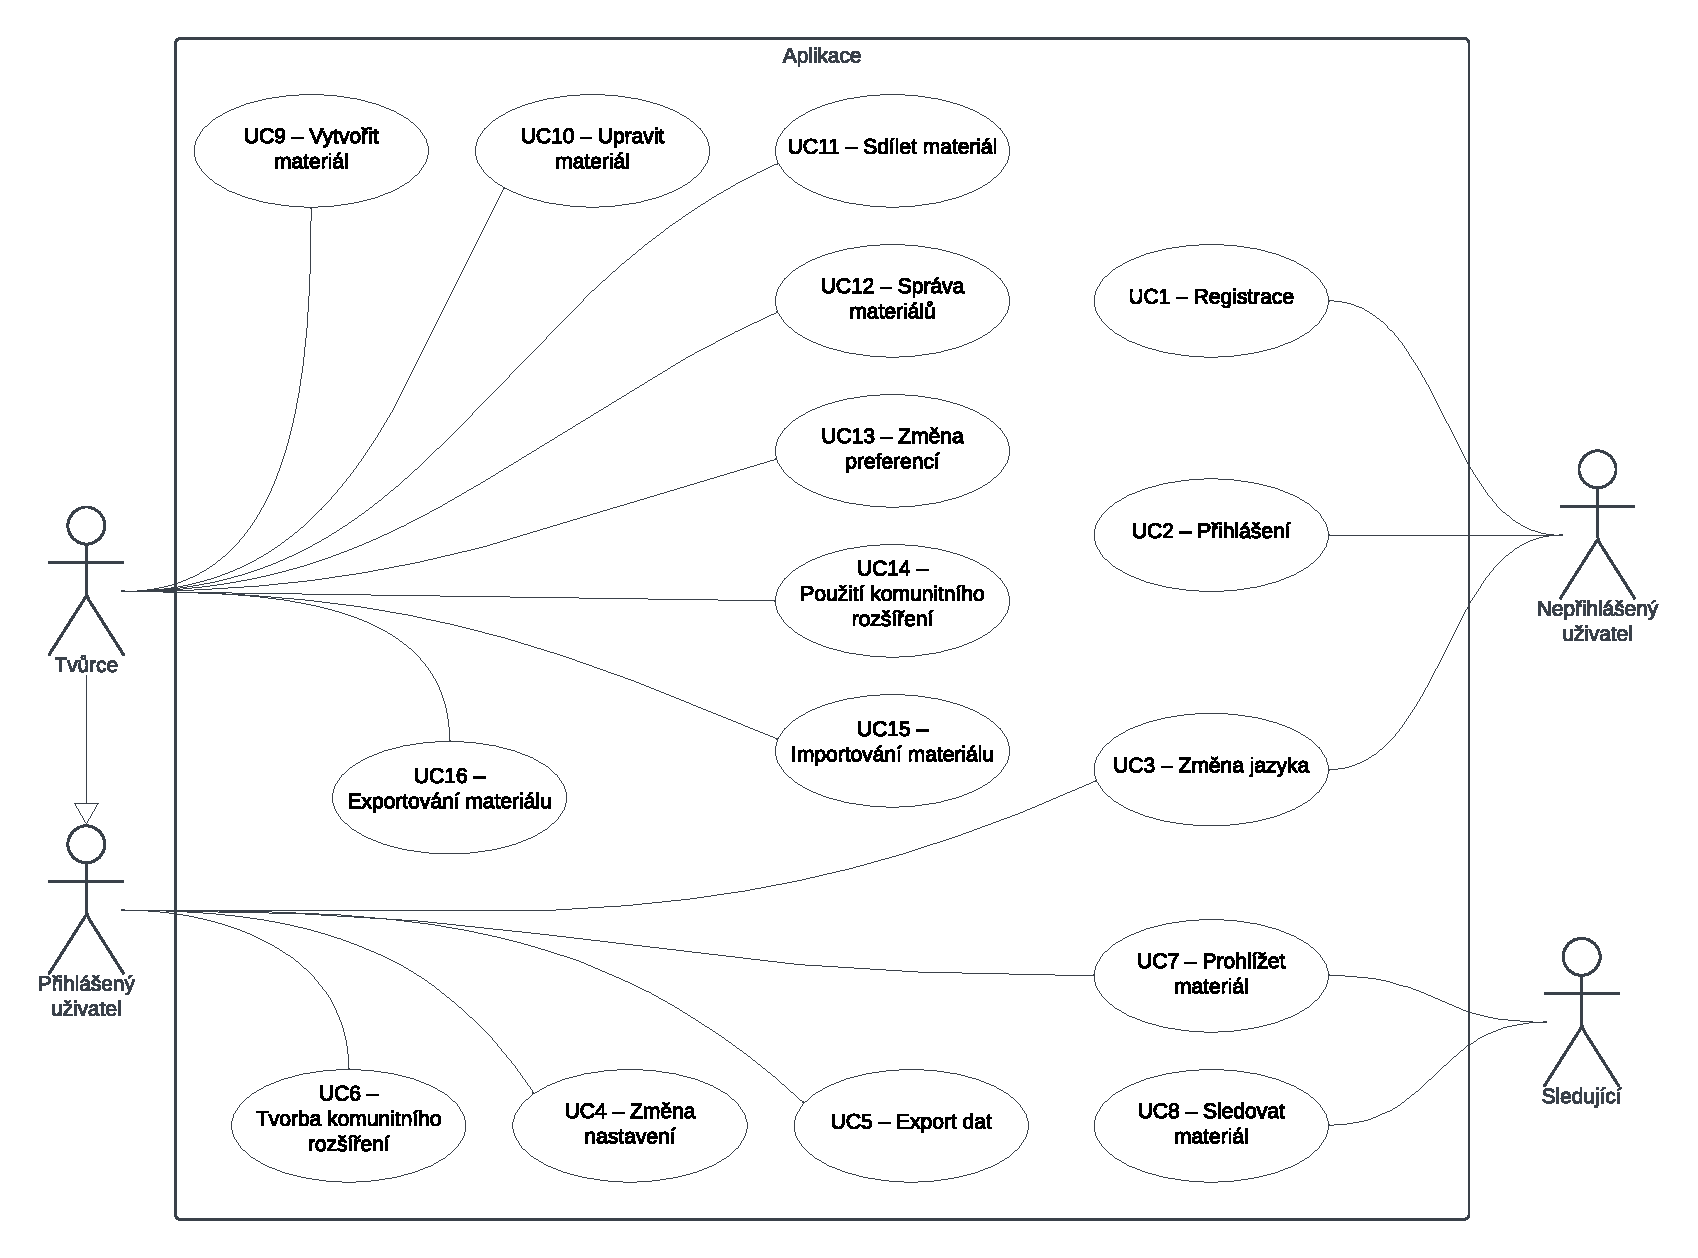
\includegraphics[width=1\textwidth]{media/03_analyza/uzivatelske_pripady.pdf}
    \caption{Diagram uživatelských případů}\label{fig:uzivatelskePripady}
\end{figure}

Níže jsou definovány všechny případy užití, které mají být implementovány ve výsledné aplikaci z~této práce.
Vztahy a propojení s~jednotlivými aktéry jsou k~dispozici na obrázku~\ref{fig:uzivatelskePripady}.

\begin{description}
    \item[UC1 -- Registrace]
    Uživatel se zaregistruje pomocí e-mailu a hesla. Po registraci je vyžadováno potvrzení e-mailové adresy prostřednictvím zaslaného ověřovacího odkazu.

    \item[UC2 -- Přihlášení]
    Uživatel se může přihlásit pomocí e-mailu a hesla. Alternativně lze použít ověření přes e-mail, kdy je na zadaný e-mail zaslán jednorázový přihlašovací kód.
    
    \item[UC3 -- Změna jazyka]
    Uživatel může změnit jazyk aplikace. Aplikace se následně přepne do zvoleného jazyka. 

    \item[UC4 -- Změna nastavení]
    Uživatel může měnit svá uživatelská nastavení, jako je heslo, e-mail a další osobní údaje.
    
    \item[UC5 -- Export dat]
    Uživatel může v~aplikaci požádat o~export dat, tedy, že obdrží archív, ve kterém je záloha všech dat, která si o~něm a jeho materiálech aplikace ukládá.
    
    
    \item[UC6 -- Tvorba komunitního rozšíření]
    Uživatel může vytvářet vlastní komunitní rozšíření pro editor a přehrávač materiálů. Tato rozšíření se píší ve skriptovacím jazyce a dovolují uživateli poslouchat různé akce, vytvářet bloky a upravovat je.
    
    \item[UC7 -- Prohlížet materiál]
    Uživatel může procházet dostupné a ukázkové materiály. Musí mít možnost přecházet mezi jednotlivými snímky, interagovat s~interaktivními prvky, přepnout na celou obrazovku, provádět pohyb v~materiálu a další související akce.
    
    \item[UC8 -- Sledovat materiál]
    Uživatel může získat odkaz ke sledování materiálu, tedy, že bude mít s~prezentujícím synchronizovaný obsah materiálu, aktuální snímek a další.
    
    \item[UC9 -- Vytvořit materiál]
    Uživatel může vytvořit nový materiál buď od začátku, nebo duplikací existujícího materiálu.
    
    \item[UC10 -- Upravit materiál]
    Uživatel může provádět komplexní úpravy materiálu pomocí vestavěného editoru. Upravování je rozděleno do několika dílčích případů:
        
        \begin{description}
            \item[UC5.1 -- Správa snímků]
            Uživatel může přidávat více snímků, měnit jejich pořadí a upravovat jejich velikost.
            
            \item[UC5.2 -- Přidání bloku]
            Uživatel může přidávat jednotlivé bloky nebo skupiny bloků. Obsah může být čerpán z~banky zdrojů, například GIF nebo obrázků.
            
            \item[UC5.3 -- Úprava vlastností bloku]
            Uživatel může měnit pro jednotlivé bloky jejich vlastnosti, zobrazení, grafické zobrazení a specifické vlastnosti bloků. U~interaktivních bloků lze definovat specifické akce, které se spustí při určité události (např. kliknutí, časovač, ...). Možné je také upravovat proměnné, nastavovat podmínky a další interaktivní chování.
            
            \item[UC5.4 -- Správa bloků]
            Uživatel může bloky označovat, kopírovat, mazat, přesouvat, seskupovat a provádět další operace.
            
            \item[UC5.5 -- Přidat média]
            Uživatel může nahrávat a vkládat vlastní obsah do prezentace.
            
            \item[UC5.6 -- Historie]
            Uživatel má přístup k~historii úprav, může se pohybovat zpět a vpřed v~provedených změnách.
        \end{description}
    
    \item[UC11 -- Sdílet materiál]
    Uživatel může nastavit viditelnost materiálu v~různých režimech (nepřihlášený, pouze přihlášení uživatelé, soukromý). Lze definovat způsob procházení materiálu (automatický, ruční, pouze interaktivitou). Dále může povolit procházení materiálů jako plátna či jako prezentaci. Materiál lze sdílet v~módu sledování.
    
    \item[UC12 -- Správa materiálů]
    Uživatel může spravovat své materiály, zobrazit seznam, vyhledávat a provádět různé akce, včetně mazání materiálů.
    
    \item[UC13 -- Změna preferencí]
    Uživatel může v~aplikaci upravovat specifické chování a nastavení editoru, způsob ukládání a způsob používání jednotlivých operací.

    \item[UC14 -- Použití komunitního rozšíření]
    Uživatel může instalovat a spravovat komunitní rozšíření, která umožňují přidávání nových funkcí do editoru.
    
    \item[UC15 -- Importování materiálu]
    Uživatel může importovat soubory v~různých formátech pro vytvoření nového materiálu.
    
    \item[UC16 -- Exportování materiálu]
    Uživatel může exportovat svůj materiál do různých formátů (např. PDF, obrázky, interaktivní formáty) pro sdílení a archivaci. Tato sdílení z~důvodu nespolupracujících formátů budou velmi omezená svou funkcionalitou a vzhledem.
\end{description}

\renewcommand{\c}{\checkmark}

\begin{table}[ht!]
\centering
\caption[Matice pokrytí funkčních požadavků]{~Matice pokrytí funkčních požadavků}\label{tabular:maticePokryti}
\begin{tabular}{l|c|c|c|c|c|c|c}
     ~         & F1 & F2 & F3 & F4 & F5 & F6 & F7 \\\hline\hline
     UC1       & \c &    &    &    &    &    &    \\\hline
     UC2       & \c &    &    &    &    &    &    \\\hline
     UC3       & \c &  &  &    &    &    &    \\\hline
     UC4       & \c &  &    &    &    &    &    \\\hline
     UC5       & \c & \c &   &   &   & \c &    \\\hline
     UC6       & \c & \c & \c & \c &    & \c &    \\\hline
     UC7       & \c & \c &    & \c &    &    &    \\\hline
     UC8       & \c & \c&    & \c &    &    & \c\tablefootnote{Ve smyslu synchronizace.} \\\hline
     UC9       & \c & \c & \c &    &  &  &  \\\hline
     UC10      & \c & \c & \c &    & \c & \c & \c \\\hline
     UC11      & \c & \c & \c &    & \c &    &    \\\hline
     UC12      & \c & \c & \c &    &    & \c &    \\\hline
     UC13      & \c & \c & \c &    &    & \c &    \\\hline
     UC14      & \c & \c & \c & \c & \c & \c & \c \\\hline
     UC15      & \c & \c &    & \c &    &    & \c \\\hline
     UC16      & \c & \c &    & \c &    &    & \c \\
\end{tabular}
\end{table}



Matice pokrytí určuje~\cite{uml_2007}, které funkční požadavky jsou nezbytné pro realizaci uživatelských případů. 
Zajišťuje kontrolu, zda každý funkční požadavek odpovídá alespoň jednomu uživatelskému případu a zda jsou pro každý uživatelský případ definovány všechny potřebné funkční požadavky. 
Pro tuto analýzu jsem sestavil matici pokrytí funkčních požadavků (viz tabulka~\ref{tabular:maticePokryti}).

\section{Doménový model}\label{text:analyza/datovymodel}

Pro lepší porozumění vztahům mezi jednotlivými prvky v~aplikaci je nutné vytvořit doménový model. 
Tento model znázorňuje~\cite{uml_2007}, jak jsou entity vzájemně propojeny a jaká data uchovávají. 
Na základě doménového modelu lze následně navrhnout databázový model. 
Diagram doménového modelu je uveden na obrázku~\ref{fig:domenovyModel}. 
Níže jsou popsány klíčové entity tohoto modelu.

\begin{description}
    \item[Uživatel] 
    Entita reprezentující uživatele systému. Obsahuje informace jako jméno a příjmení, e-mailovou adresu, hašované heslo, stav aktivace, aktivační token, datum vytvoření účtu, datum posledního přihlášení a datum poslední změny hesla.

    \item[Žádost o~přihlášení] 
    Entita uchovávající kód žádosti o~přihlášení, jeho expiraci a stav použití, o~které požádal konkrétní uživatel.
    
    \item[Žádost o~export]
    Entita reprezentující žádost uživatele o~export osobních údajů z~platformy.
    
    \item[Preference] 
    Reprezentuje uživatelská nastavení editoru. Obsahuje možnosti ukládání, frekvenci ukládání, velikost historie a specifické funkce editoru. Vytváří se při vytvoření uživatele v~aplikaci.

    \item[Soubor] 
    Entita popisující soubory nahrané do systému. Obsahuje mimo jiné název, MIME typ, velikost, typ úložiště a umístění souboru. Mohou se používat v~konkrétních blocích materiálů.
    
    \item[Materiál] 
    Reprezentuje obsah vytvářený uživatelem. Obsahuje název, datum vytvoření a datum poslední úpravy. Obsahuje jednotlivé snímky.
    
    \item[Nastavení] 
    Definuje nastavení materiálu. Například se jedná o~viditelnost k~ostatním uživatelům, spolu editoři, způsob procházení, mód procházení, čas přechodu.
    
    \item[Snímek] 
    Každý materiál obsahuje snímky, které představují jednotlivé části obsahu. Entita obsahuje náhledový obrázek a pozici v~rámci materiálu. Obsahuje taktéž data, která udávají nastavení snímku, např. velikost a šířku, a dále obsahuje bloky materiálu.
    
    \item[Blok] 
    Základní stavební prvek snímku. Obsahuje atributy jako typ, pozici, velikost, rotaci, přiřazenou skupinu, vrstvu, stav zamknutí a interaktivitu. Má další specifické vlastnosti v~závislosti na konkrétním typu bloku. Například se může jednat o~text, obrázek či komplexní blok pro zobrazení kódu
    
    \item[Rozšíření]
    Reprezentuje rozšíření v~platformě. Je navázán na autora rozšíření a verze. Verze je konkrétní verze kódu.
\end{description}

\begin{figure}[ht!]
    \centering
    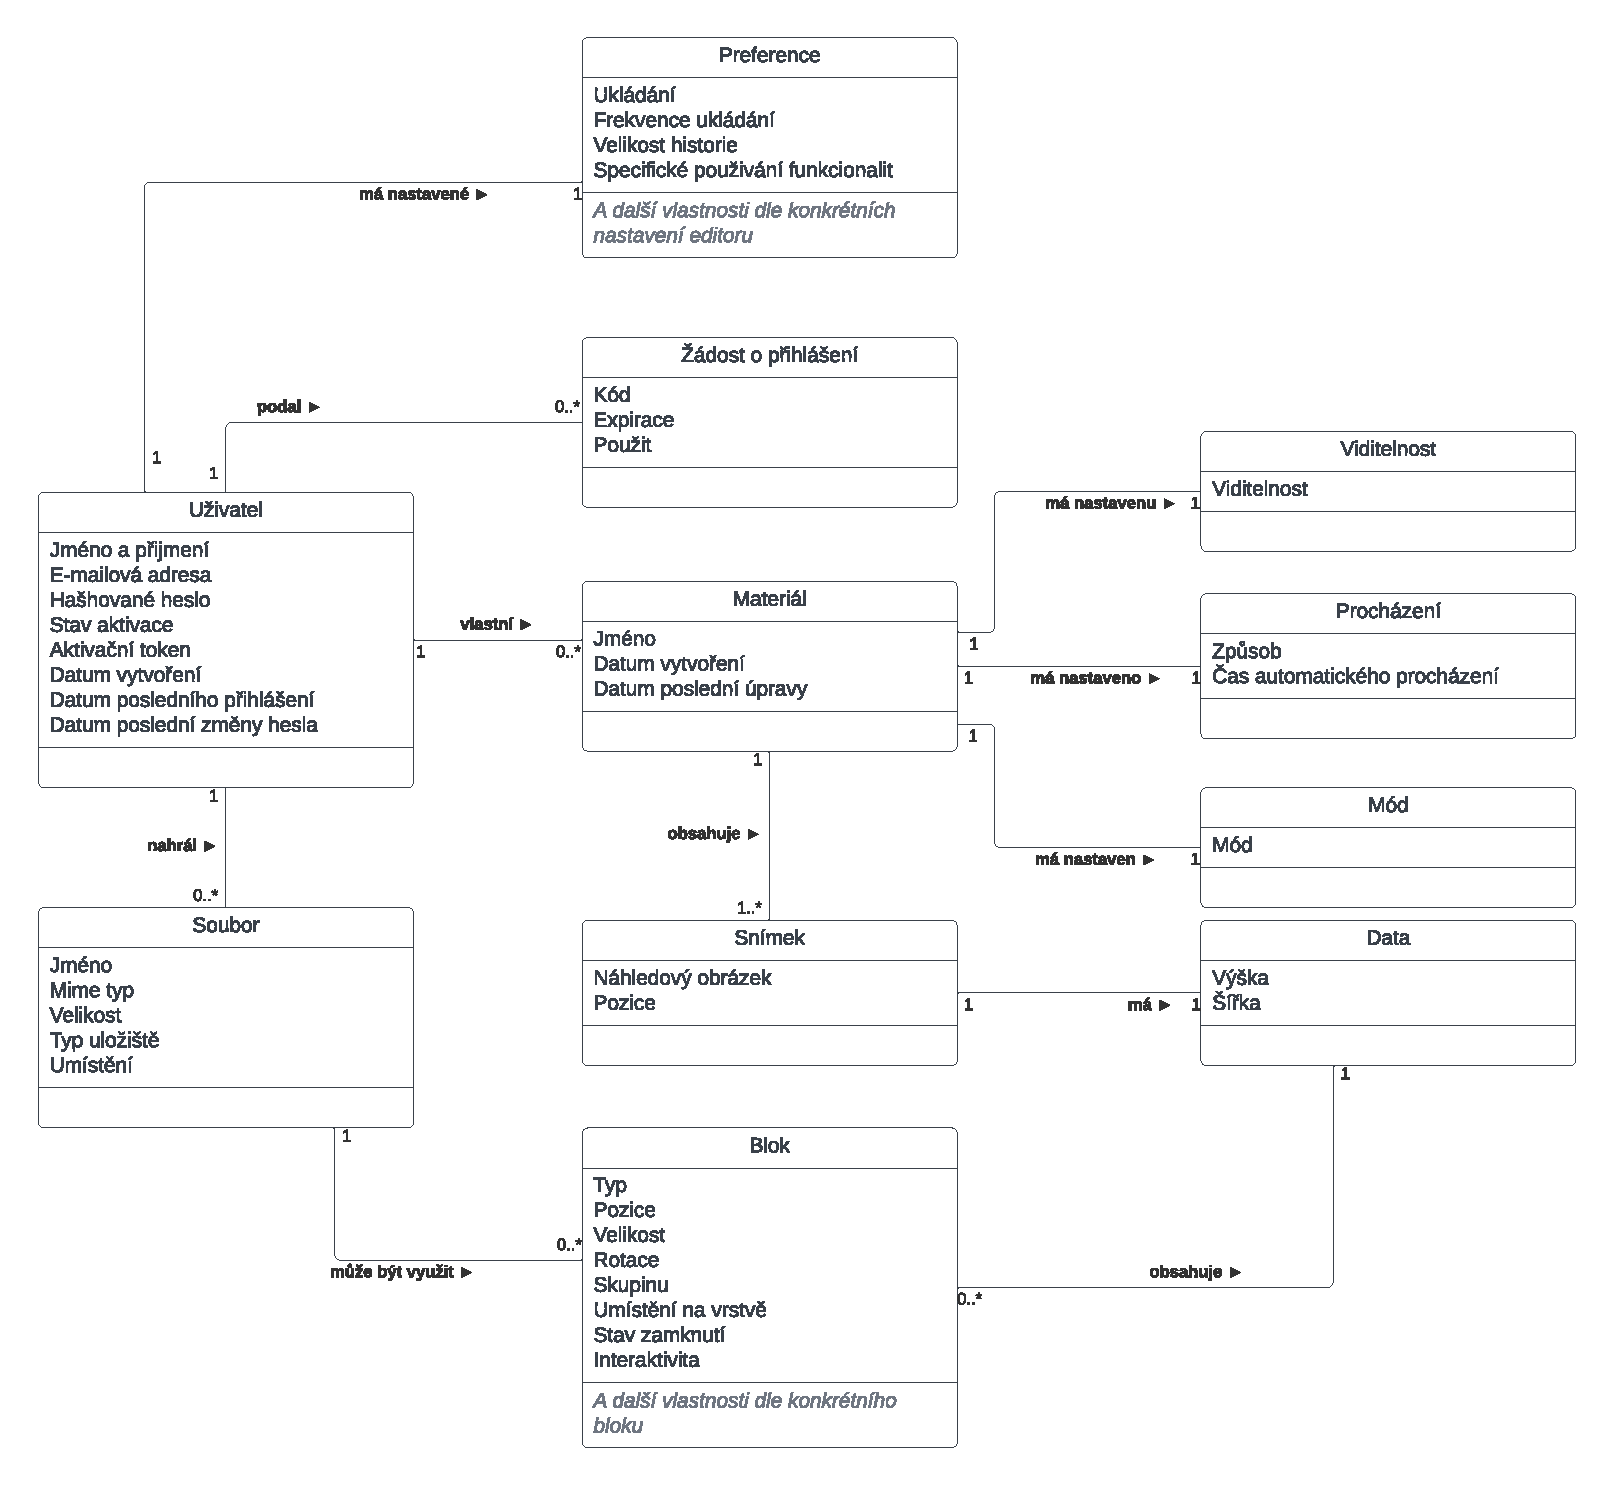
\includegraphics[width=1\textwidth]{media/03_analyza/domenovy_model.pdf}
    \caption{Diagram doménového modelu}\label{fig:domenovyModel}
\end{figure}